\documentclass{beamer}

\usetheme{Warsaw}
\definecolor{indigo(web)}{rgb}{0.29, 0.0, 0.51}
\usecolortheme[named=indigo(web)]{structure}

\title[Improving reproducibility in building simulation]{Improving reproducibility in building simulation: a pure-Python approach to geometry creation}
\author{Steven Firth}
\institute{Loughborough University}
\date{2021-06-23}

\begin{document}
	
	\begin{frame}
		\maketitle
	\end{frame}
	
	\begin{frame}{My background}
		\begin{itemize}
			\item I joined Loughborough University in 2008
			\item My job title is Reader in Building Performance Modelling
			\item I teach building simulation, energy data analysis, sustainable building design and renewable energy.
			\item I was a member of the University's Open Research Working Group in 2019.
			\item I was awarded the CALIBRE Winter 2019 Award for Open Research
			\item In 2015 I published the Refit Smart Home dataset on the University's Data Repository (14,307 views, 3,997 downloads)
			\item I publish papers on FAIR data and open research methods using Python and Jupyter Notebooks 
			\item I maintain the GitHub pages for the Building Energy Research Group
			
		\end{itemize}
	\end{frame}
	
	\begin{frame}{The problem I am trying to solve}
		\begin{itemize}
			\item I would construct a building simulation model of a 4 bed house and to simulate the energy performance of the house using the EnergyPlus software.
			\item I would like to do this in an open, transparent way so that the whole process is reproducible. 
		\end{itemize}
	\end{frame}

	\begin{frame}{What is "Reproducible"?}
		The Alan Turing Institute in its publication 'The Turing Way' defines reproducible research for data science as: \\ [10pt]
		\begin{quote}
			Work that can be independently recreated from the same data and the same code that the original team used. 
		\end{quote}
	\end{frame}

	\begin{frame}{An Example of Reproducibility}
		This presentation is reproducible as it is written in code (Latex)\\[10pt]
		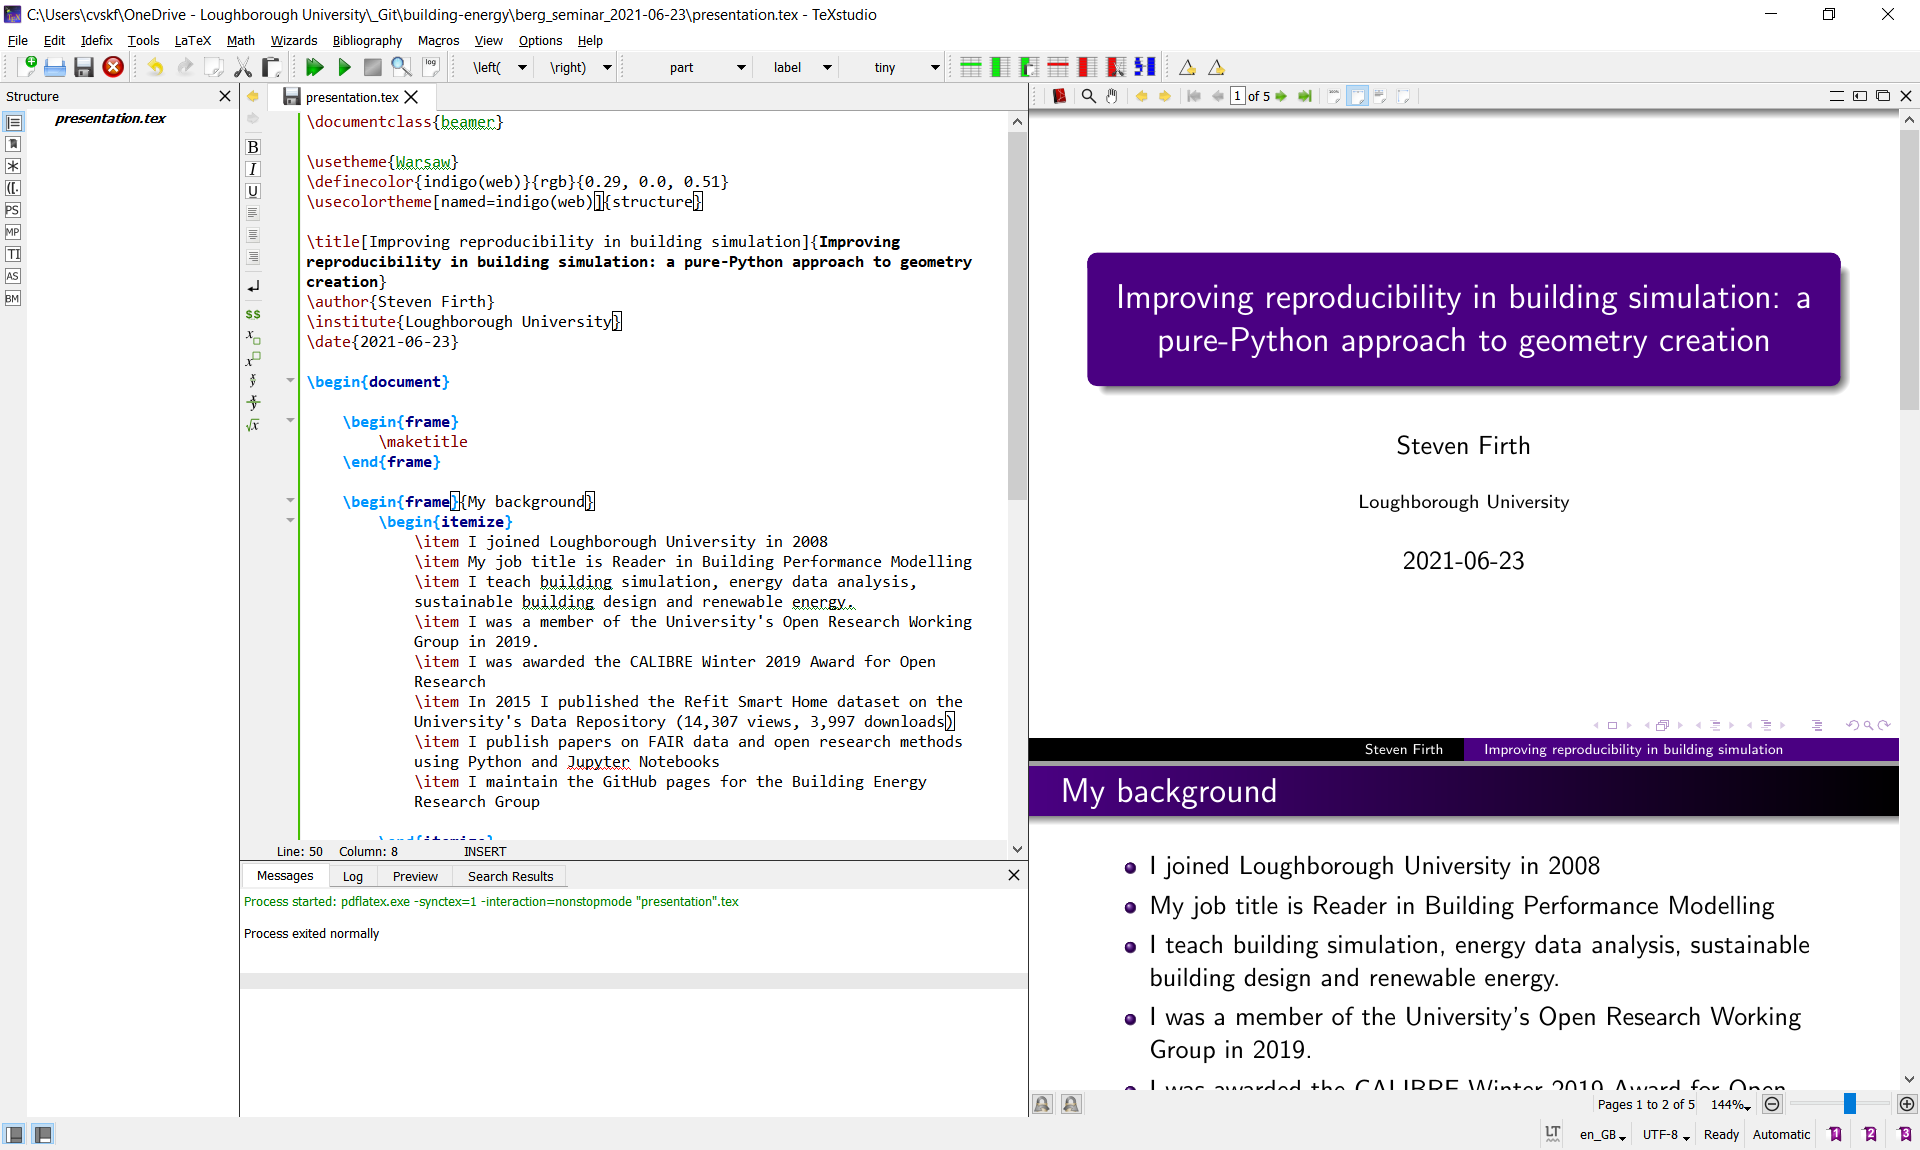
\includegraphics[width=\textwidth,keepaspectratio]{latex_example.png}
	\end{frame}
	
	\begin{frame}{An Example of Open Reproducibility}
		This presentation is also open as the code is hosted on the BERG Github repository\\[10pt]
		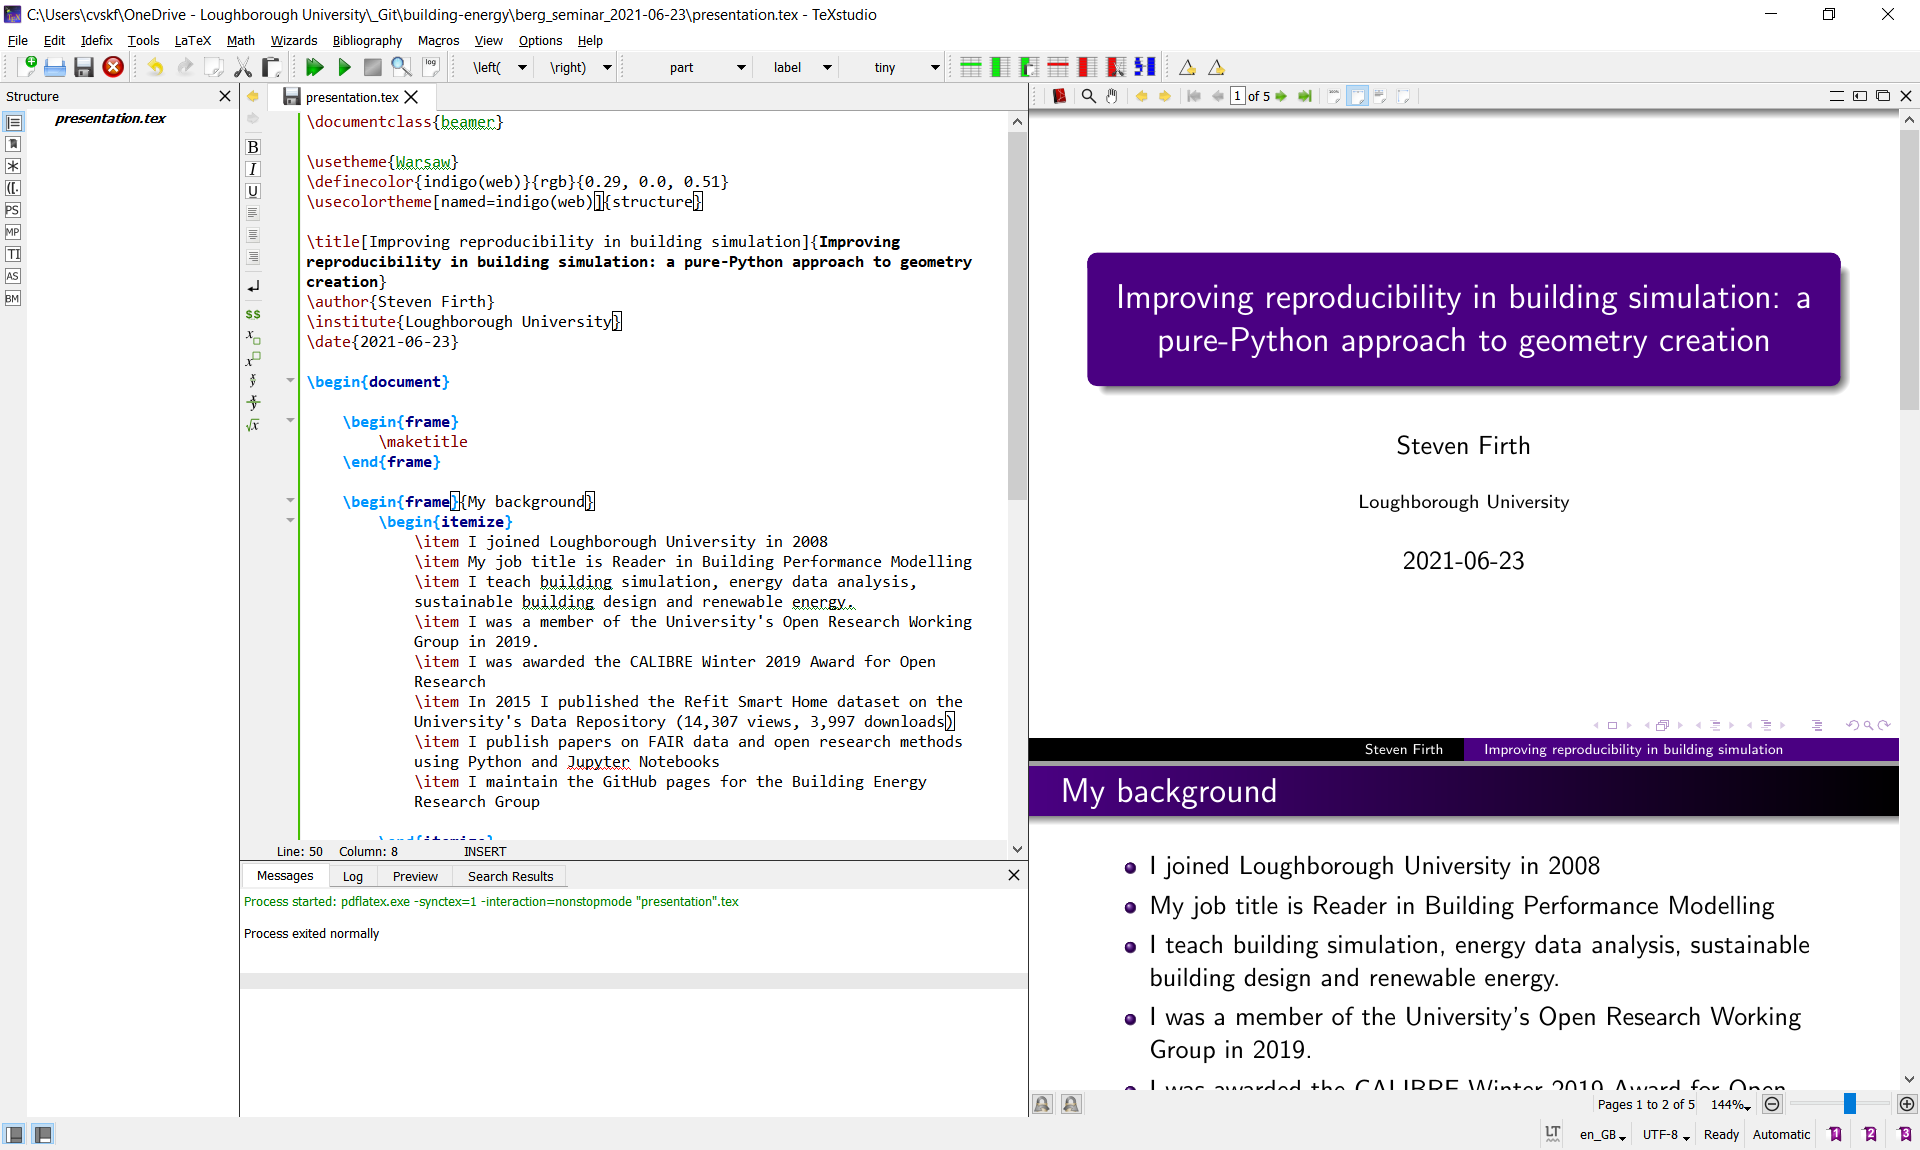
\includegraphics[width=\textwidth,keepaspectratio]{latex_example.png}
	\end{frame}
	
\end{document}